\documentclass{sigchi}

% Use this section to set the ACM copyright statement (e.g. for
% preprints).  Consult the conference website for the camera-ready
% copyright statement.

% Copyright
\CopyrightYear{2018}
%\setcopyright{acmcopyright}
\setcopyright{acmlicensed}
%\setcopyright{rightsretained}
%\setcopyright{usgov}
%\setcopyright{usgovmixed}
%\setcopyright{cagov}
%\setcopyright{cagovmixed}
% DOI
\doi{http://dx.doi.org/10.475/123_4}
% ISBN
\isbn{123-4567-24-567/08/06}
%Conference
\conferenceinfo{CHI'16,}{May 07--12, 2016, San Jose, CA, USA}
%Price
\acmPrice{\$15.00}

% Use this command to override the default ACM copyright statement
% (e.g. for preprints).  Consult the conference website for the
% camera-ready copyright statement.

%% HOW TO OVERRIDE THE DEFAULT COPYRIGHT STRIP --
%% Please note you need to make sure the copy for your specific
%% license is used here!
% \toappear{
% Permission to make digital or hard copies of all or part of this work
% for personal or classroom use is granted without fee provided that
% copies are not made or distributed for profit or commercial advantage
% and that copies bear this notice and the full citation on the first
% page. Copyrights for components of this work owned by others than ACM
% must be honored. Abstracting with credit is permitted. To copy
% otherwise, or republish, to post on servers or to redistribute to
% lists, requires prior specific permission and/or a fee. Request
% permissions from \href{mailto:Permissions@acm.org}{Permissions@acm.org}. \\
% \emph{CHI '16},  May 07--12, 2016, San Jose, CA, USA \\
% ACM xxx-x-xxxx-xxxx-x/xx/xx\ldots \$15.00 \\
% DOI: \url{http://dx.doi.org/xx.xxxx/xxxxxxx.xxxxxxx}
% }

% Arabic page numbers for submission.  Remove this line to eliminate
% page numbers for the camera ready copy
% \pagenumbering{arabic}

% Load basic packages
\usepackage{balance}       % to better equalize the last page
\usepackage{graphics}      % for EPS, load graphicx instead 
\usepackage[T1]{fontenc}   % for umlauts and other diaeresis
\usepackage{txfonts}
\usepackage{mathptmx}
\usepackage[pdflang={en-US},pdftex]{hyperref}
\usepackage{color}
\usepackage{booktabs}
\usepackage{textcomp}

% Some optional stuff you might like/need.
\usepackage{microtype}        % Improved Tracking and Kerning
% \usepackage[all]{hypcap}    % Fixes bug in hyperref caption linking
\usepackage{ccicons}          % Cite your images correctly!
% \usepackage[utf8]{inputenc} % for a UTF8 editor only

% If you want to use todo notes, marginpars etc. during creation of
% your draft document, you have to enable the "chi_draft" option for
% the document class. To do this, change the very first line to:
% "\documentclass[chi_draft]{sigchi}". You can then place todo notes
% by using the "\todo{...}"  command. Make sure to disable the draft
% option again before submitting your final document.
\usepackage{todonotes}

% Paper metadata (use plain text, for PDF inclusion and later
% re-using, if desired).  Use \emtpyauthor when submitting for review
% so you remain anonymous.


\def\plaintitle{The Language Learning of the Future: Personal, Interesting, Adaptive}

% The Textbook of the Present: Personal, Adaptable, Interesting
% The Textbook for the Generation Y: Contextual, Personal, Adaptable
% The Language Learning of the Present: Personal, Interesting, Adaptive


\def\plainauthor{First Author, Second Author, Third Author,
  Fourth Author, Fifth Author, Sixth Author}
\def\emptyauthor{}
\def\plainkeywords{Authors' choice; of terms; separated; by
  semicolons; include commas, within terms only; required.}
\def\plaingeneralterms{Documentation, Standardization}

% llt: Define a global style for URLs, rather that the default one
\makeatletter
\def\url@leostyle{%
  \@ifundefined{selectfont}{
    \def\UrlFont{\sf}
  }{
    \def\UrlFont{\small\bf\ttfamily}
  }}
\makeatother
\urlstyle{leo}

% To make various LaTeX processors do the right thing with page size.
\def\pprw{8.5in}
\def\pprh{11in}
\special{papersize=\pprw,\pprh}
\setlength{\paperwidth}{\pprw}
\setlength{\paperheight}{\pprh}
\setlength{\pdfpagewidth}{\pprw}
\setlength{\pdfpageheight}{\pprh}

% Make sure hyperref comes last of your loaded packages, to give it a
% fighting chance of not being over-written, since its job is to
% redefine many LaTeX commands.
\definecolor{linkColor}{RGB}{6,125,233}
\hypersetup{%
  pdftitle={\plaintitle},
% Use \plainauthor for final version.
%  pdfauthor={\plainauthor},
  pdfauthor={\emptyauthor},
  pdfkeywords={\plainkeywords},
  pdfdisplaydoctitle=true, % For Accessibility
  bookmarksnumbered,
  pdfstartview={FitH},
  colorlinks,
  citecolor=black,
  filecolor=black,
  linkcolor=black,
  urlcolor=linkColor,
  breaklinks=true,
  hypertexnames=false
}

% create a shortcut to typeset table headings
% \newcommand\tabhead[1]{\small\textbf{#1}}

\usepackage{xspace}

\newcommand{\stcnt}{sixty\xspace}

% End of preamble. Here it comes the document.
\begin{document}

\title{\plaintitle}

\numberofauthors{3}
\author{%
  \alignauthor{Leave Authors Anonymous\\
    \affaddr{for Submission}\\
    \affaddr{City, Country}\\
    \email{e-mail address}}\\
  \alignauthor{Leave Authors Anonymous\\
    \affaddr{for Submission}\\
    \affaddr{City, Country}\\
    \email{e-mail address}}\\
  \alignauthor{Leave Authors Anonymous\\
    \affaddr{for Submission}\\
    \affaddr{City, Country}\\
    \email{e-mail address}}\\
}

\maketitle

%!TEX root=paper.tex

\begin{abstract}
  UPDATED---\today. 

  This paper describes the implementation and 
  deployment of a system that supports learners
  of a foreign language in reading materials that
  are both personally interesting and at the right 
  difficulty level. 

  The system provides translations for the unknown 
  words at the touch of the screen while at the same
  time monitoring the current state of the knowledge
  of the learner in order to be able to estimate the  
  texts of the appropriate difficulty.

  This paper reports on the results of deploying the
  system for one month with \stcnt Dutch highschool students 
  learning French. 
  The students were very positive about the system, 
  and their teacher has decided to redeploy the sytem
  for the next academic year.

\end{abstract}

\category{H.5.m.}{Information Interfaces and Presentation
  (e.g. HCI)}{Miscellaneous} \category{See
  \url{http://acm.org/about/class/1998/} for the full list of ACM
  classifiers. This section is required.}{}{}

\keywords{\plainkeywords}


\newpage
\section{Introduction}

It is well known that free reading is one of the best ways of improving the vocabulary. The Internet contains vast amounts of information in all the possible languages that somebody would want to learn. However, there are two problems with allowing a reader to read materials on the internet: 
\begin{itemize}
  \item The materials might be too difficult for them
  \item The reading tools might not be appropriate
\end{itemize}

Moreover, textbooks usually come with exercises at the end of a text. However, if one allows the readers to read whatever they like: how are they going to do exercises? Can we generate exercises that are tailored based on the past experience of students free reading?



%!TEX root=paper.tex

\newpage
\section{The System}

For the long term, we envision an open educational ecosystem in which different creators can integrate their applications by interacting with a core API that provides the basic contextual translations, user knowledge estimation, and recommendations for words to be studied and texts to be read \cite{Lungu16}. 

However, in order to bootstrap, experiment with, and show the potential of such an ecosystem, we present here our basic implementation of each of the components. In particular we describe our own implementation of: 

\begin{description}

  \item [Text Recommender] -- which consists of a feed subscription mechanism, an article browser that presents the results of crawling the selected feeds that the user is interested in

  \item [Text Reader] -- which is a web-based interactive text reader which provides seamless in place translations
  
  \item [Vocabulary Trainer] -- which consists of an exercise platform which generates exercises based on a reader's past reading experience

\end{description}

The components that we present here are implemented using HTML5 and Javascript technologies for the front end and Python and Flask for the backend. For the frontend, we have experienced in the past with writing native applications, however, the interaction with the native elements was too clumsy. Moreover, maintaining multiple systems for multiple platforms is too expensive for an academic environment. The decision turned out to be practical since the users of our system come from multiple platforms.


\subsection{The Text Recommender}
\ml{make sure that this flows well for the reader while also keeping it short}
The reading recommender is simple at the moment. It consists of a Feed Subscription and an Article Browser.

\subsubsection{Feed Subscription}
When the user indicates that they would like to subscribe to a new source, as explained above, the subscription dialog is displayed. Zeeguu categorizes feeds by their language, and thus we allow users to select any language available and retrieve a list of that language's sources. Languages are represented by flags, as their compact and iconic representation should be universally understood.

\begin{figure}[h!]
\centering
  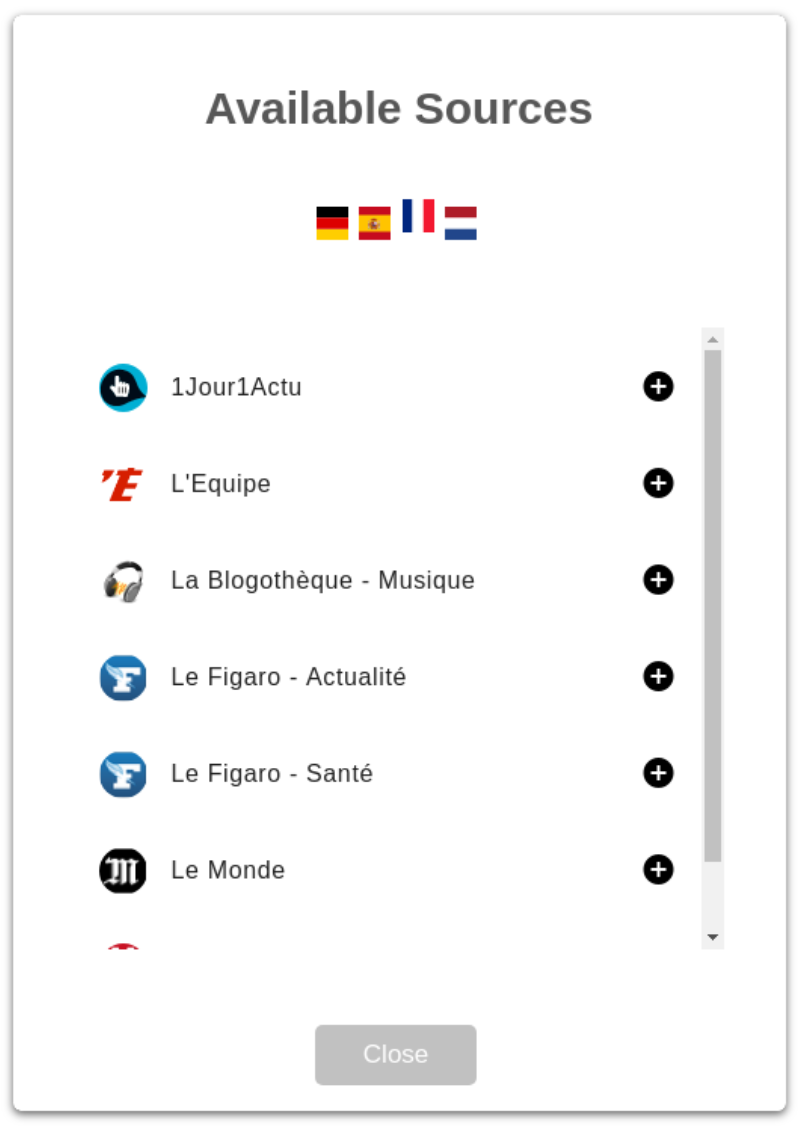
\includegraphics[width=0.4\columnwidth]{figures/available_sources}
  \caption{Different users subscribe to different sources}~\label{fig:system_subscriptions}
\end{figure}


\subsubsection{Article Browser}

Article listing presents the source, a summary of the article, and an estimated difficulty level of the article.

In order to properly visualize the reading difficulty of an article in an intuitive manner, there are three levels of information displayed here. First we display a flag representing the language of the article. This is so because a learner could be actually registered to feeds in multiple languages. Second, we allow the user to rapidly judge difficulty on an intuitive level by color coding the difficulty from green to yellow to red. When a particular article has grasped the user's attention, we allow for a more cognitive judgment by scoring the article from 0 to 5 in difficulty.

\ml{TODO: write about how is difficulty estimation done currently}

\begin{figure}[h!]
\centering
  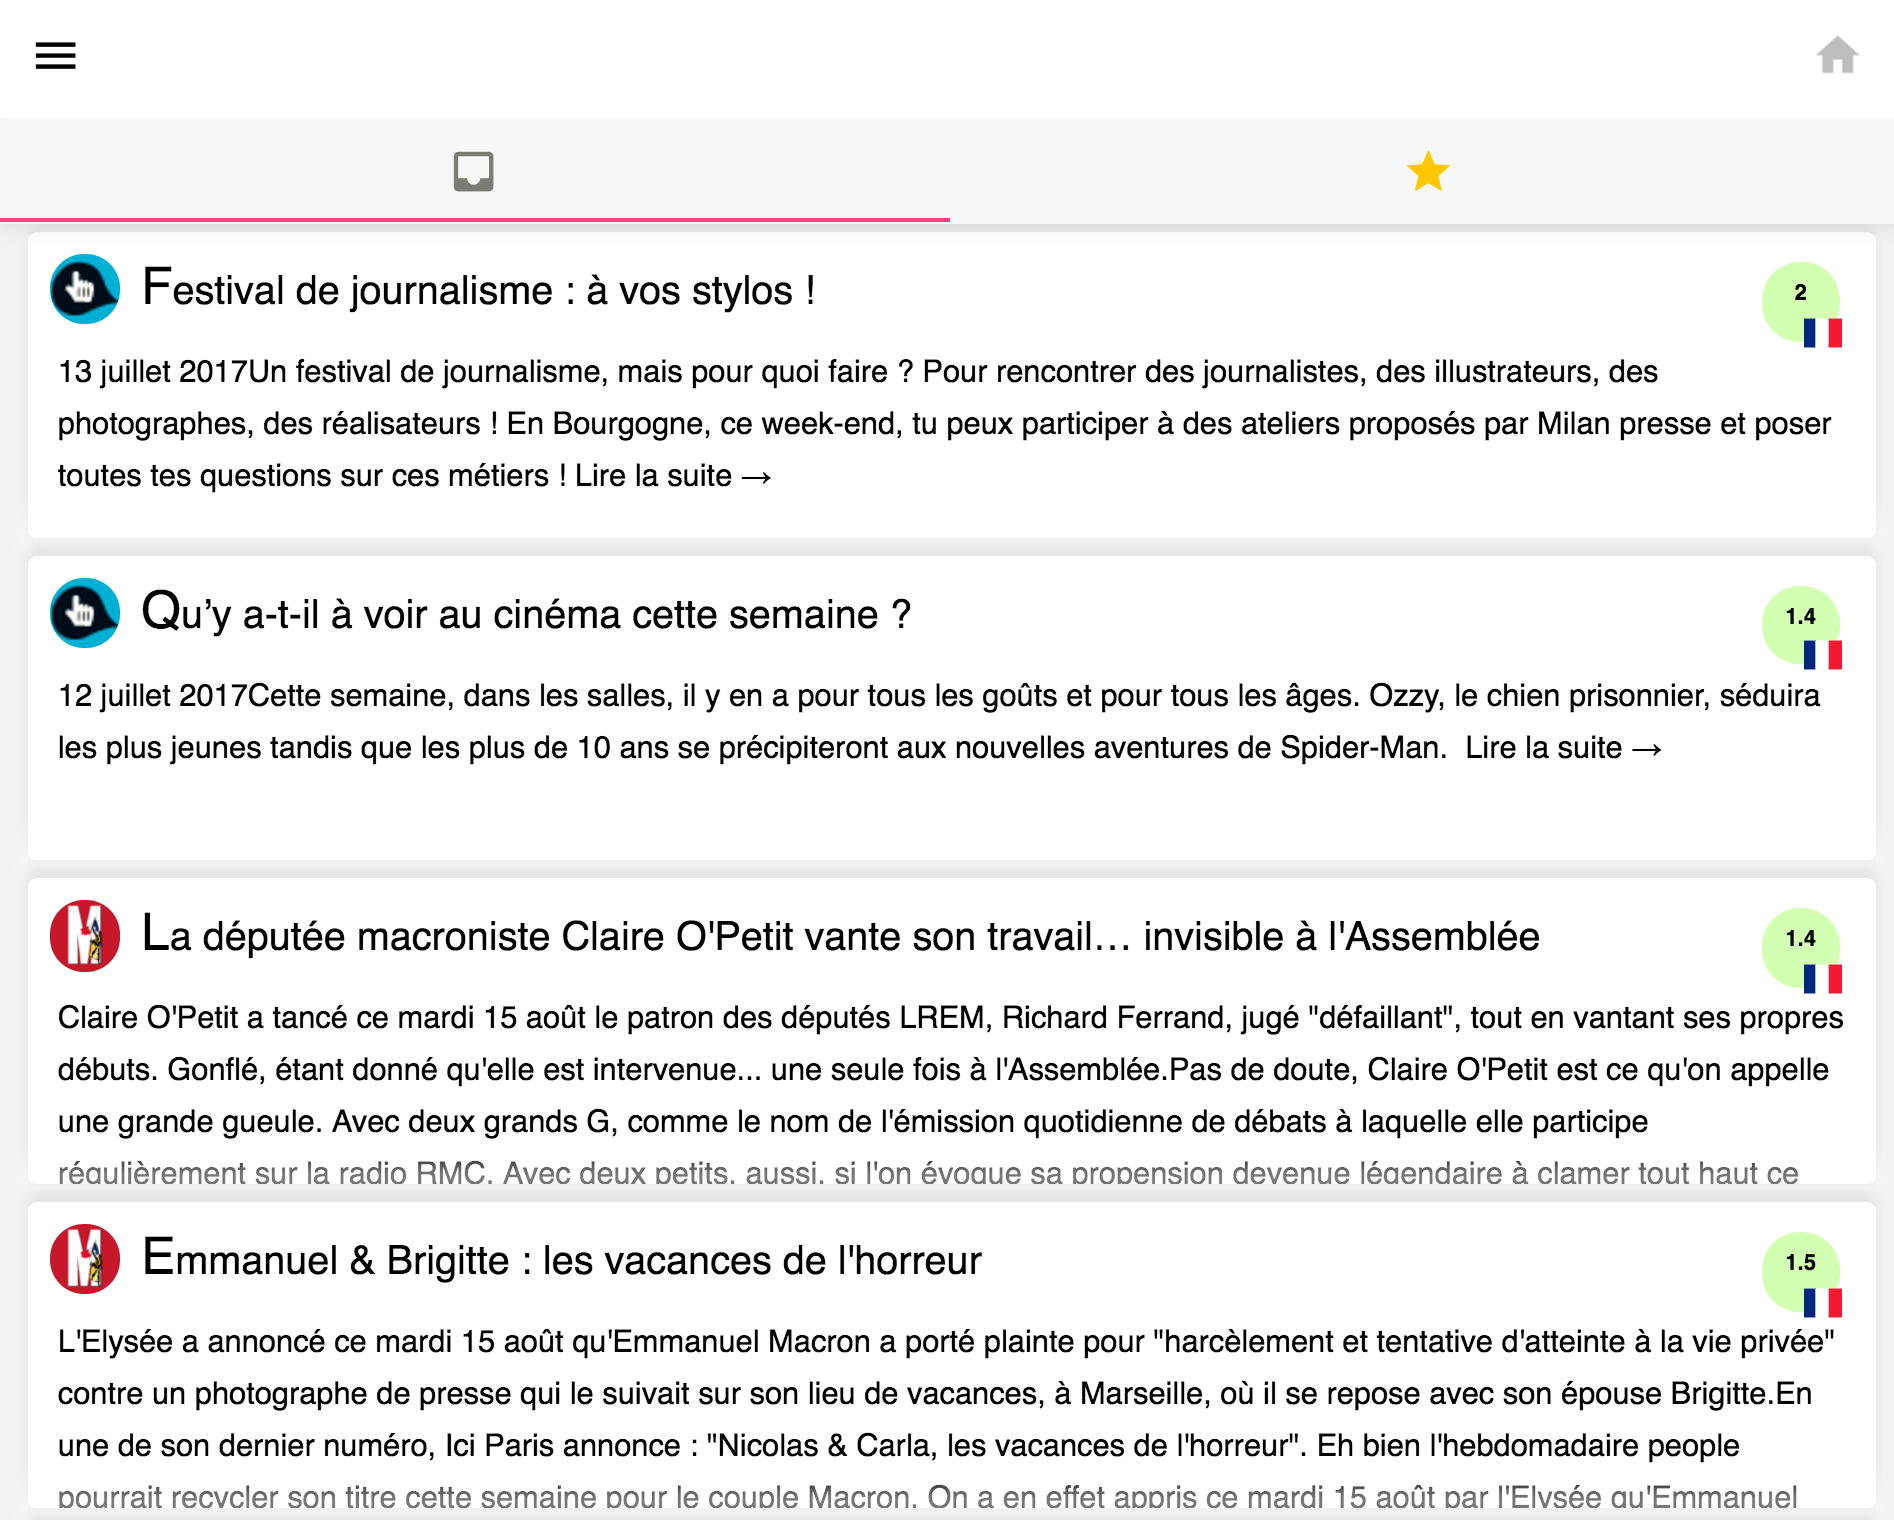
\includegraphics[width=0.95\columnwidth]{figures/article_listing}
  \caption{Article listing presents the source, a summary of the article, and an estimated difficulty level of the article }~\label{fig:registrations}
\end{figure}


\subsection{The Text Reader}

The goal of the reader is to make reading as facile as possible. To do this we optimized for the most frequent action that a reader might want to perform. Translating a word. 

We explored several types of interactions and we settled on the following: a user clicks on a word, a translation is inserted right after the word, as Figure \ref{fig:translated_word} illustrates: 

\begin{figure}[h!]
\centering
  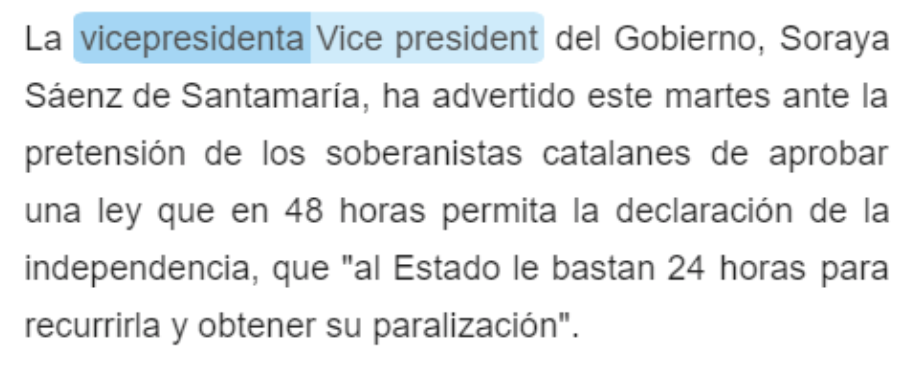
\includegraphics[width=0.8\columnwidth]{figures/translated_word}
  \caption{A translated word is inserted after the tapped word.}~\label{fig:translated_word}
\end{figure}

Ohter alternatives that we explored and eventually dropped for each had disadvantages were: 
\begin{itemize}

  \item Showing a popup of the translation, and then hiding it again. This had the disadvantage of in the case of a more difficult sentence the reader forgetting the word at the begining of the sentence by the time he arrived to the end, and having to re-translate it. 

  \item Piggybacking on the native selection mechanism. We experimented with allowing the learner to select a word in the same way this is normally done on the corresponding platform and to add the translation as an option in the corresponding popup menu. The problem with this is that native selection is slow, requiring about one second before it is activated. 
\end{itemize}


\subsubsection{Chaining Multiple Adjacent Translations}
The user can chain a few consecutive words into a single translation by simply tapping adjacent words which are automatically merged in a translation bubble (Figure \ref{fig:translation_extension}). This is useful for collocations and in cases where by expanding the translated set of words the precision of the translation increases. 

    \begin{figure}[h!]
    \centering
      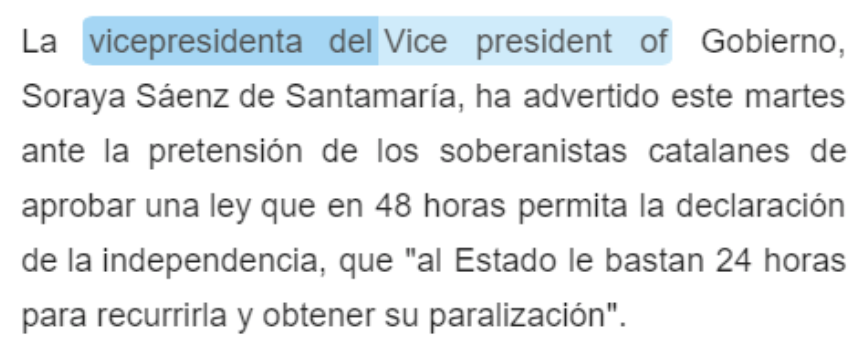
\includegraphics[width=0.8\columnwidth]{figures/translated_words1}
      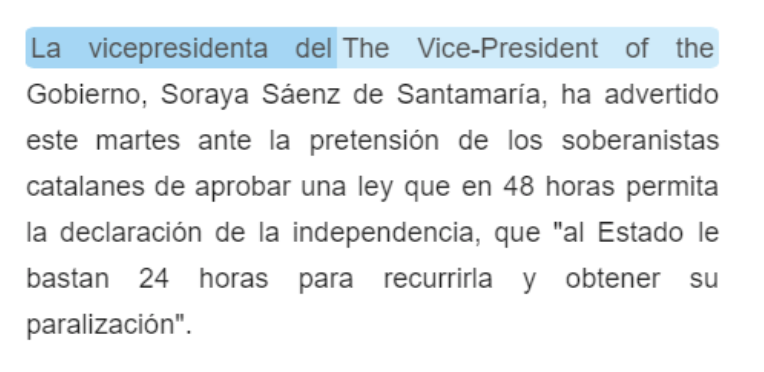
\includegraphics[width=0.8\columnwidth]{figures/translated_words2}
      \caption{When adjacent words are tapped the translation bubble is extended accordingly}~\label{fig:translation_extension}
    \end{figure}

This minimalistic interaction model serves a double purpose - it enables and eases the translation of several chained words but it discourages users from translating entire sentences or phrases. This is good because it is in line with the recommendations of the literature (e.g. Renandya argues that extensive reading should discourage intensive use of translations\cite{renadya07-power}) but also because it reduces the amount of characters which are being translated by the learner (and thus the costs of the system, since some of the translation services have a per-character fee). 

One of the limitations of this interaction is that it is not clear (at least at the moment) how to expand it for the situations in which expressions are present that are composed of words which are not adjacent (e.g. particle verbs in German and Dutch).


\subsubsection{Alternate Translations}
Due to the limitations of machine translations, it can be the case that multiple translations might seem appropriate in a context. In such a case the system will insert the most likely alternative but allow the reader to discover the others. With a click on the translation, a drop-down menu appears in which alternatives are presented. Besides the alternatives, there's also an input box in which the learner can provide his own version if none of the offered alternatives are correct. 

Based on telemetry from the system it seems that \ml{must check and limit this only to the french-learning kids} the alternative translations menu is opened one in every eight translations. 

\begin{figure}[h!]
\centering
  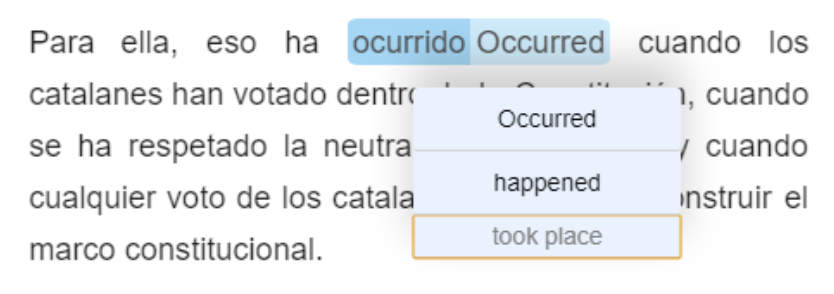
\includegraphics[width=0.8\columnwidth]{figures/translation_alter_menu}
  \caption{A translated word is inserted after the tapped word.}~\label{fig:registrations}
\end{figure}

\subsubsection{Pronounciation}
One of the important features, which was suggested by early beta-testers and added to the system after that, was the option of having pronounciation of the given word. Currently this is the action associated with tapping on the highlighted translated word. Although no user has yet complained about it, this means that a user can not pronounce a word without it being translated first. It might also be that for some languages this is more important than for others, and we just did not have users learning those languages (e.g. Danish is notoriously hard to pronounce). In the future we plan to expand the interaction modes to allow pronounciation to exist seperately from translation.

\subsection{The Vocabulary Trainer}

Given the list of words that a user does not know we can generate exercises for them based on their past readings.

The various interactive elements (IEs) that are present in this exercise (and in some of the other exericses are): 

\begin{description}
	\item [A hint button (IE1)] will present the user with the correct answer.
	\item [Check the answer (IE2)] will verify the correctness of the answer.
	\item [Word pronunciation (IE3)] will sound the pronounciation.
	\item [Control (IE4)] over the exercise card allows for reporting or deleting the exercise.
	\item [Input box (IE5)] allows for entering a solution.
\end{description}

\begin{figure}[h!]
\centering
  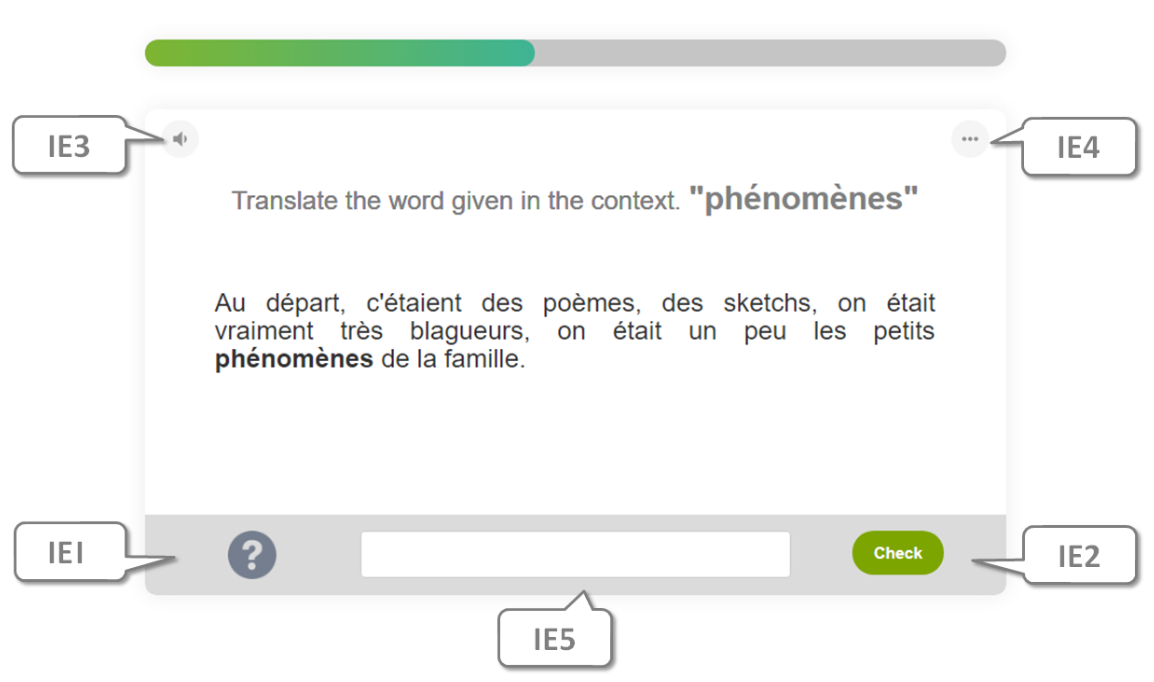
\includegraphics[width=\columnwidth]{figures/exercise_translate}
  \caption{One of the exercise types with which the user is presented. Multiple exercise types are taken from the users past reading context}
\end{figure}

\subsubsection{Words Good for Study}

The words good for study are the ones that are either starred by the user, or are important and of quality based on a set of heuristics. 

\begin{description}

  \item [Important words] are the ones which appear frequently in the language. 
  
  \item [Quality words] are most of the times single words or at most two adjacent words. They come with a context which is not too short but not too long. 

\end{description}

\subsubsection{Scheduling Exercises}

The scheduling algorithm is based on an adaptive, response-time-based scheduling algorithm [was developed] to increase the efficiency of perceptual learning by Mettler et al. \cite{Mettler14-ARTS}. After evaluating several alternative scheduling strategies we settled on the Mettler one since it has been proven to have gains with both familiar, seen items as well as with new, unseen instances and the benefits of adaptive scheduling were present at an immediate test as well as at a delay \cite{Mettler14-ARTS}.



One of the problems with this is that sometimes the context is too long and sometimes 


\subsection{Translation Service}

The translations are provided by our server. The main advantage of this indirection is that this allows the server to track the words that are looked up and the context (sentence) in which they are being looked up. This information is then used for estimating learner knowledge and for generating later personalied exercises. 

To avoid depending on a single service and to also increase the likelihood that at least one of the alternative translations is the correct one, the translation service dispatches in parallel requests to at least three third party translation APIs: Google Translate, Microsoft Translate, and Glosbe -- a free translation API. The first two provide contextual translations and multi-word translations, while the third is a simple dictionary. 

The dependency of the translation service on multiple third party APIs allows for a higher reliability and a chance to guarantee a low response time: when a service is down or too slow to respond, the results from it are ignored.

\subsection{The Teacher Dashboard}

Although not the focus of this paper, the system has also a dashboard for the teacher. The teacher can see the history of what his students have read. 







%!TEX root=paper.tex

\newpage
\section{The Students}

The population that we tested our infrastructure with represent \stcnt highschool students from Groningen in the Netherlands. Their native language is Dutch and most of them speak fluent English. 

We deployed the system with the translations in English instead of Dutch and we made it clear to the students that if for some of them this is insufficient, 

Their ages vary between ... and ... 

Their self declared language level is presented in the table below: 

At the begining of June, we visited the school, and we introduced the
way the infrastructure is to be used during one hour. 

The system was to be used until June 28th. 

The teacher asked the students to be using the infrastructure and write reports on the way they used. For evey half an hour of usage, the students would have to write a brief report that they would submit to the teacher about how they spent their time.

% To talk to Nienke about the other types of analysis we can do on this data
%!TEX root=paper.tex

\newpage
\section{Do The Readers Find Personally Interesting Articles?}

\subsection {Feed Subscriptions}
Figure \ref{fig:registrations} represents an incidence matrix collected at the end of the study interval: the columns represent students, and the rows represent news feeds; if a student is registered to a given feed, at the intersection of the corresponding row and column we place an x. 

We would expect to see fully continuous horizontal rows of data-points if every user subscribed to the same feed, and fully continuous vertical rows if every user subscribed to all of the feeds available. The notion that these patterns are largely absent in Figure 4 supports our assumption that different individuals prefer to subscribe to different reading sources.

The figure illustrates that giving the students the freedom to choose the sources they wanted, allowed each one of them to express their interest. 

\begin{figure}[h!]
\centering
  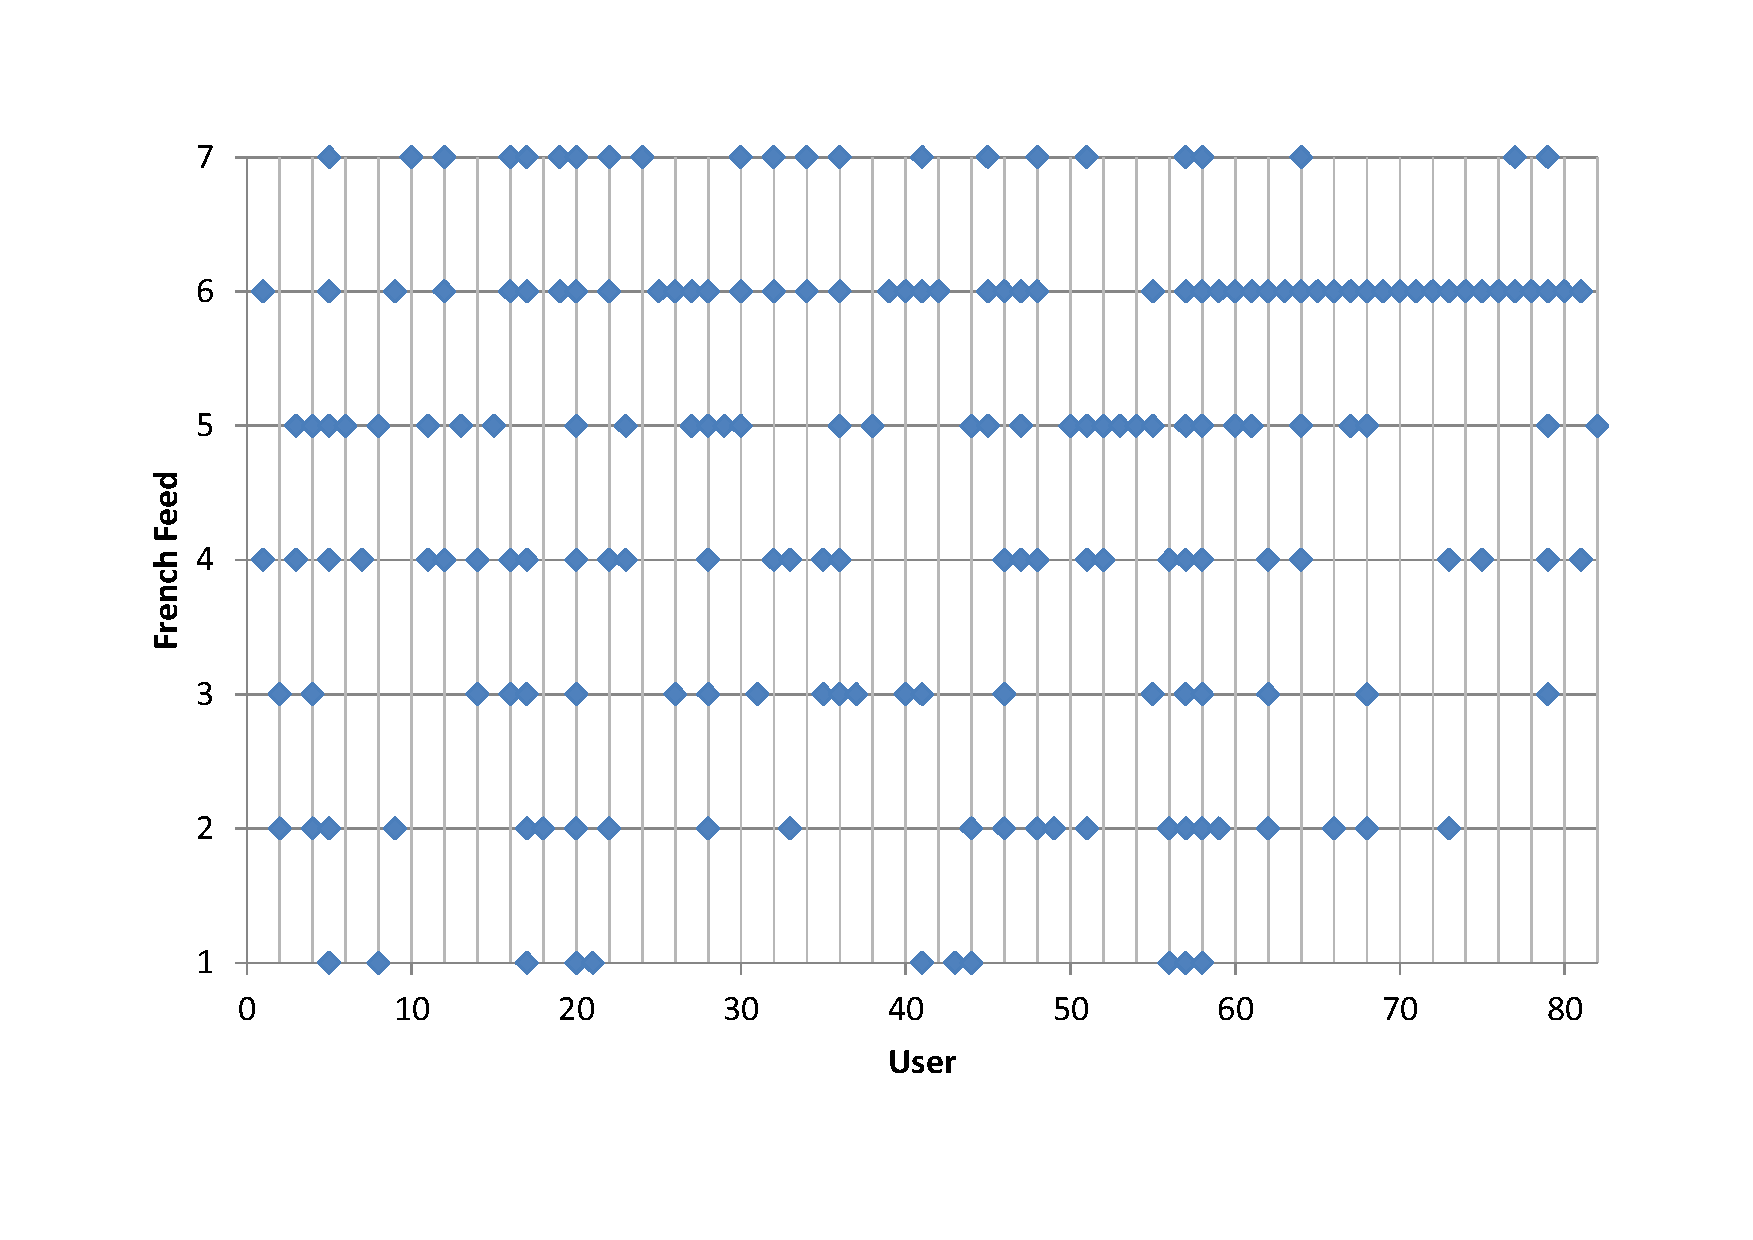
\includegraphics[width=\columnwidth]{figures/users_feeds}
  \caption{Different users subscribe to different sources}~\label{fig:registrations}
\end{figure}

Of course some feeds are more popular than others. Projecting the data- points into the vertical axis results in the histogram of Figure 5.

\begin{figure}[h!]
\centering
  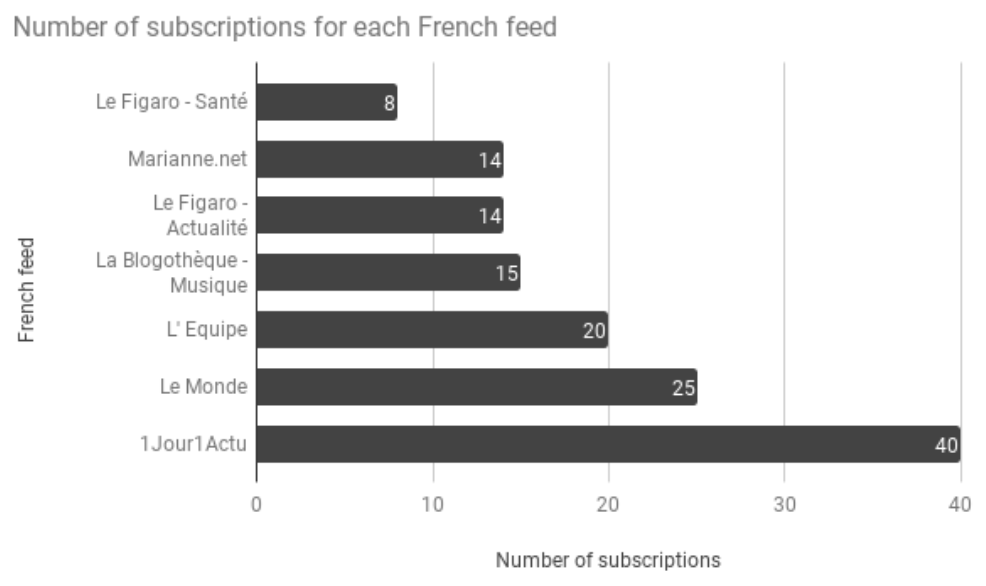
\includegraphics[width=\columnwidth]{figures/feed_popularity}
  \caption{Some feeds are more popular than others}~\label{fig:registrations}
\end{figure}


Feed {\em 1Jour1Actu} is the most popular French feed, and feed Le Figaro - Sant\'e is the least popular French feed. In order to see whether or not this might be related to how they are presented in the dialog window of our system, we can compare the order of popularity with the order in which they are displayed.

\begin{figure}[h!]
\centering
  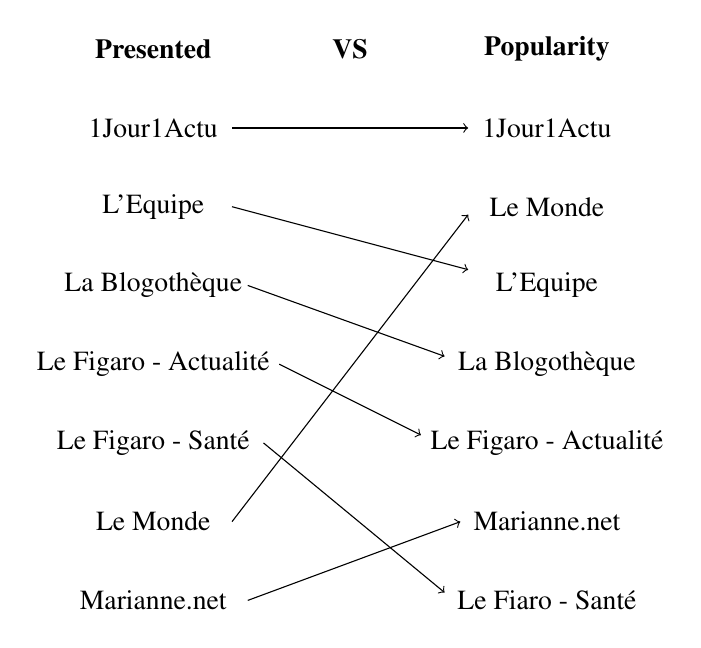
\begin{tikzpicture}[scale=1]
    % Columns.
    \node at (0  , 0) {\bf Presented};
    \node at (2.5, 0) {\bf VS};
    \node at (5  , 0) {\bf Popularity};
    
    % As presented.
    \node at (0,-1) {1Jour1Actu};
    \node at (0,-2) {L'Equipe};
    \node at (0,-3) {La Blogoth\`{e}que};
    \node at (0,-4) {Le Figaro - Actualit\'{e}};
    \node at (0,-5) {Le Figaro - Sant\'{e}};
    \node at (0,-6) {Le Monde};
    \node at (0,-7) {Marianne.net};
    
    % As popular.
    \node at (5,-1) {1Jour1Actu};
    \node at (5,-2) {Le Monde};
    \node at (5,-3) {L'Equipe};
    \node at (5,-4) {La Blogoth\`{e}que};
    \node at (5,-5) {Le Figaro - Actualit\'{e}};
    \node at (5,-6) {Marianne.net};
    \node at (5,-7) {Le Fiaro - Sant\'{e}};
    
    % Arrows between presented and popular.
    \draw [->] (1,-1)   --   (4,-1);
    \draw [->] (1,-2)   --   (4,-2.8);
    \draw [->] (1.2,-3) --   (3.7,-3.9);
    \draw [->] (1.6,-4) --   (3.4,-4.9);
    \draw [->] (1.4,-5) --   (3.7,-6.9);
    \draw [->] (1,-6)   --   (4,-2.1);
    \draw [->] (1.2,-7) --   (3.9,-6);
    
  \end{tikzpicture}
  \caption{The popularity of the feeds vs. their ranking in the UI}~\label{fig:registrations}
\end{figure}


\subsection{Article Interactions}
If we investigate the articles that the users interact with, we see the same pattern: each user explores their own interest, and there is no one article that is interesting for all of them. 

\begin{figure}[h!]
\centering
  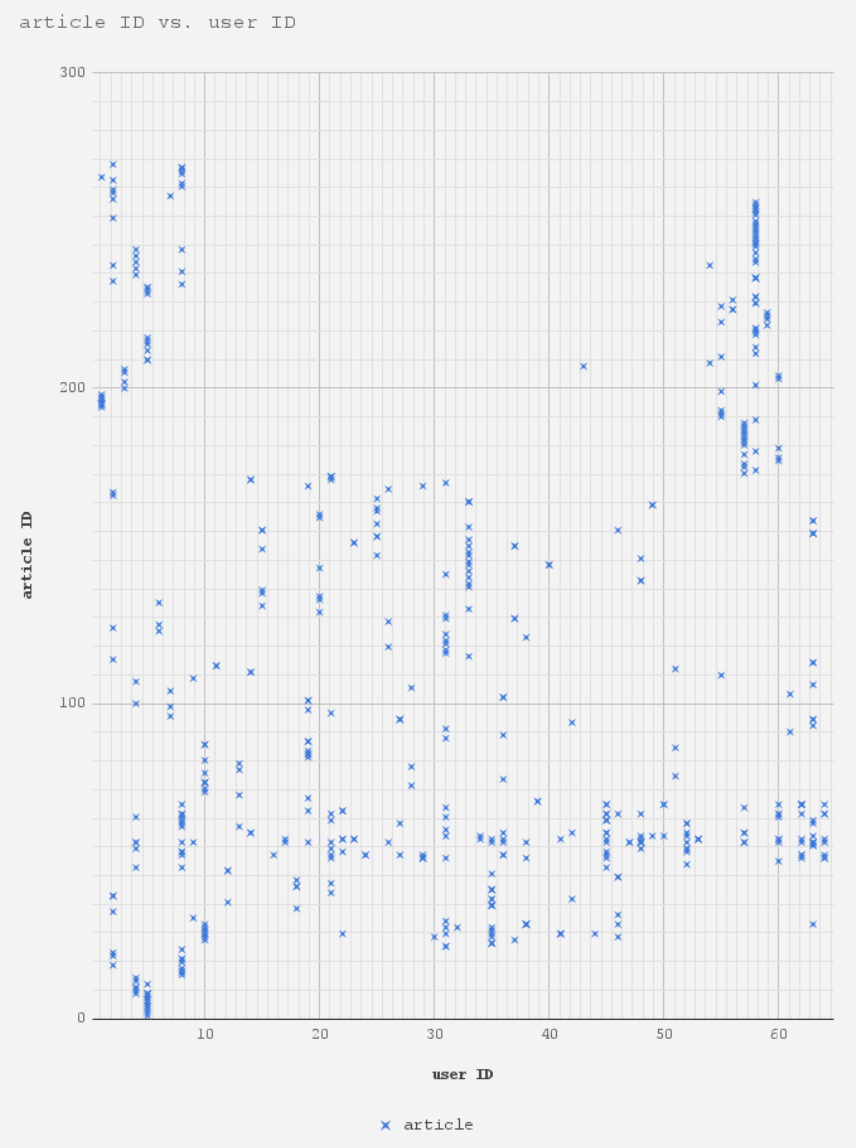
\includegraphics[width=\columnwidth]{figures/users_articles}
  \caption{Every student has their own article reading preferences}~\label{fig:registrations}
\end{figure}

\newpage
\section{Which of the Interactive Features Are Most Important When Reading?}
We tracked the usage of the various features in the interactive reader. What we see is that in average, a students requests an alternate translation for one in every eight translations. 

The third most used feature is the text to speech feature. This was a feature that was recommended by one of our expert beta-testers. 


\begin{figure}[h!]
\centering
  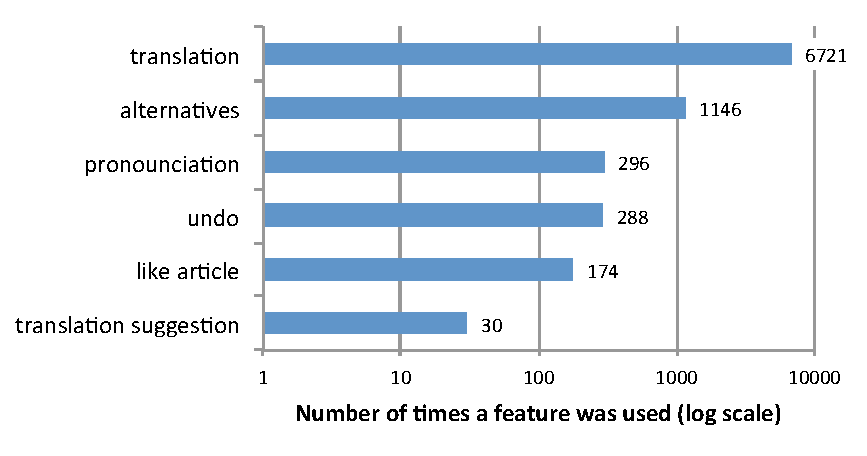
\includegraphics[width=0.7\columnwidth]{figures/reader_feature_usage}
  \caption{... }
\end{figure}

To see how widespread are the various features among our users, we also looked at 


\begin{figure}[h!]
\centering
  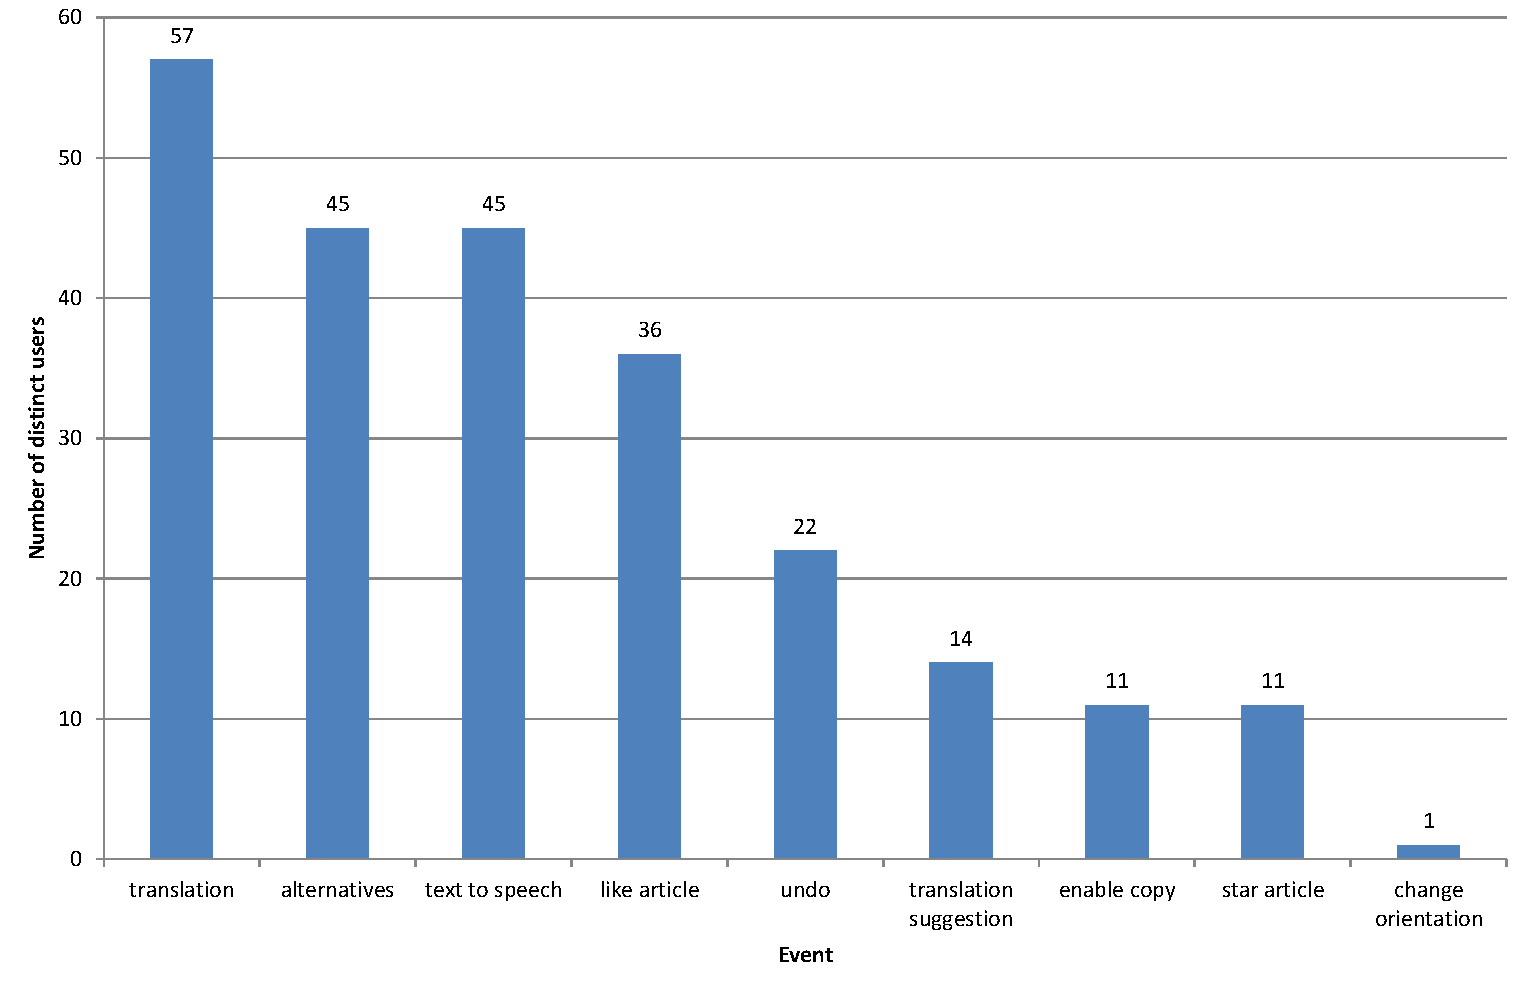
\includegraphics[width=0.9\columnwidth]{figures/reader_feature_usage_per_user}
  \caption{The usage of the various reader features by the various users }
\end{figure}

We also looked at the number of times the same word or phrase was pronounced by the same user. This data ranges from one single pronunciation to 14 pronunciations for the same word (phrase). The size of this interval is mostly due to the users’ different proficiency in a certain language and the difficulty in pronunciation of the word (phrase) itself. Nevertheless, on average, the number approaches 1.66 pronunciation requests for the same
piece of text, suggesting that users are generally sufficiently content with a pronunciation after hearing it the first time.



\section{Are the Personalized Exercises Useful?}

The personalized exercises are a complement to the reading. To show that 
users actually use them ... 

\begin{figure}[h!]
\centering
  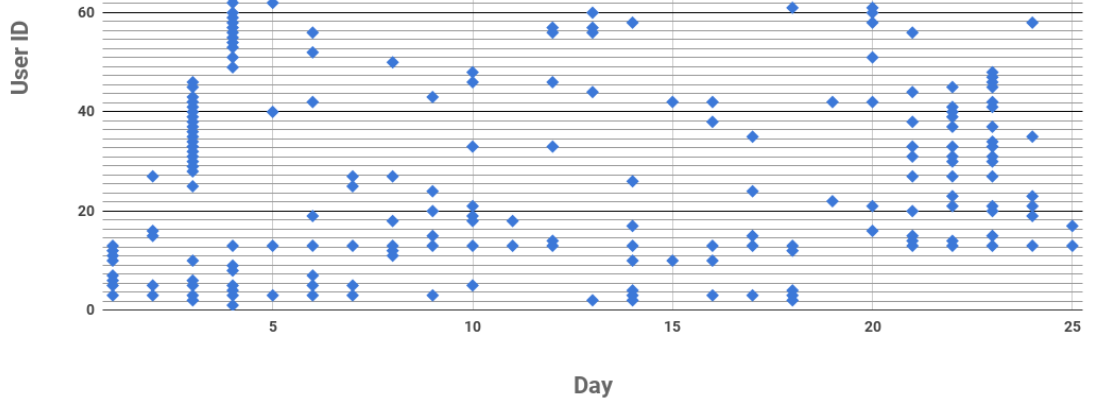
\includegraphics[width=\columnwidth]{figures/users_exercises}
  \caption{The students are doing exercises at their own pace throughout the one month interval }
\end{figure}

we could also show that they benefit from them... 



\section{User Feedback}

Besides the analysis that we did based on the observed user data, we also asked the students a series of questions, among which whether they preferred the reading platform and why. Some of the qnswers can be seen in the screenshot below. It becomes clear that the students appreciate the possibility of reading what is interesting for them.


\section{Threats to Validity}

Threat to external validity: the students that we worked with are representative we believe for the Dutch highschool student population. 

We presented a system, and we showed that it has the potential to generate user involvement. However the study we performed is not sufficient to reach a strong conclusion about the impact of the system we present... 

The feedback from the users was positive. However, they might have been influenced by our enthusiastic presentation of the system at the begining of the testing month. 

We showed that the users are using the system extensively. However, this might be because the students had to use the system as part of their assignment in the class. We showed that the majority of the students used the system constantly throughout the one month period. If they only used it for a grade, we would have expected a more focused cramming at the end of the period (which we actually saw with a few of the students, but not with the majority). 

The majority of the students who answered our post-usage survey said that  they prefer our system to a textbook. However, we still think this is not very conclusive since the number of students who answered our survey was quite limited: 12 of the 60 students represent about 20\% of the participants. 

% We observed that students prefer to interact with different texts...  

The algorithms for scheduling are the state of the art in spaced repetition. However, we did not have a control group to see whether this approach works better than others. Moreover, note that other approaches for using spaced repetition already exist; what is unique in our approach is that the students learn based on personalized exercises generated based on the context of their past readings.


\section{Availability}
The system described in this paper is deployed online and available at \url{https://zeeguu.unibe.ch}. If the reader of this article would want to test it they are invited to use the ``CHI'' code word while following the  ``Become a Betatester'' link from the homepage.

\begin{figure}[h!]
\centering
  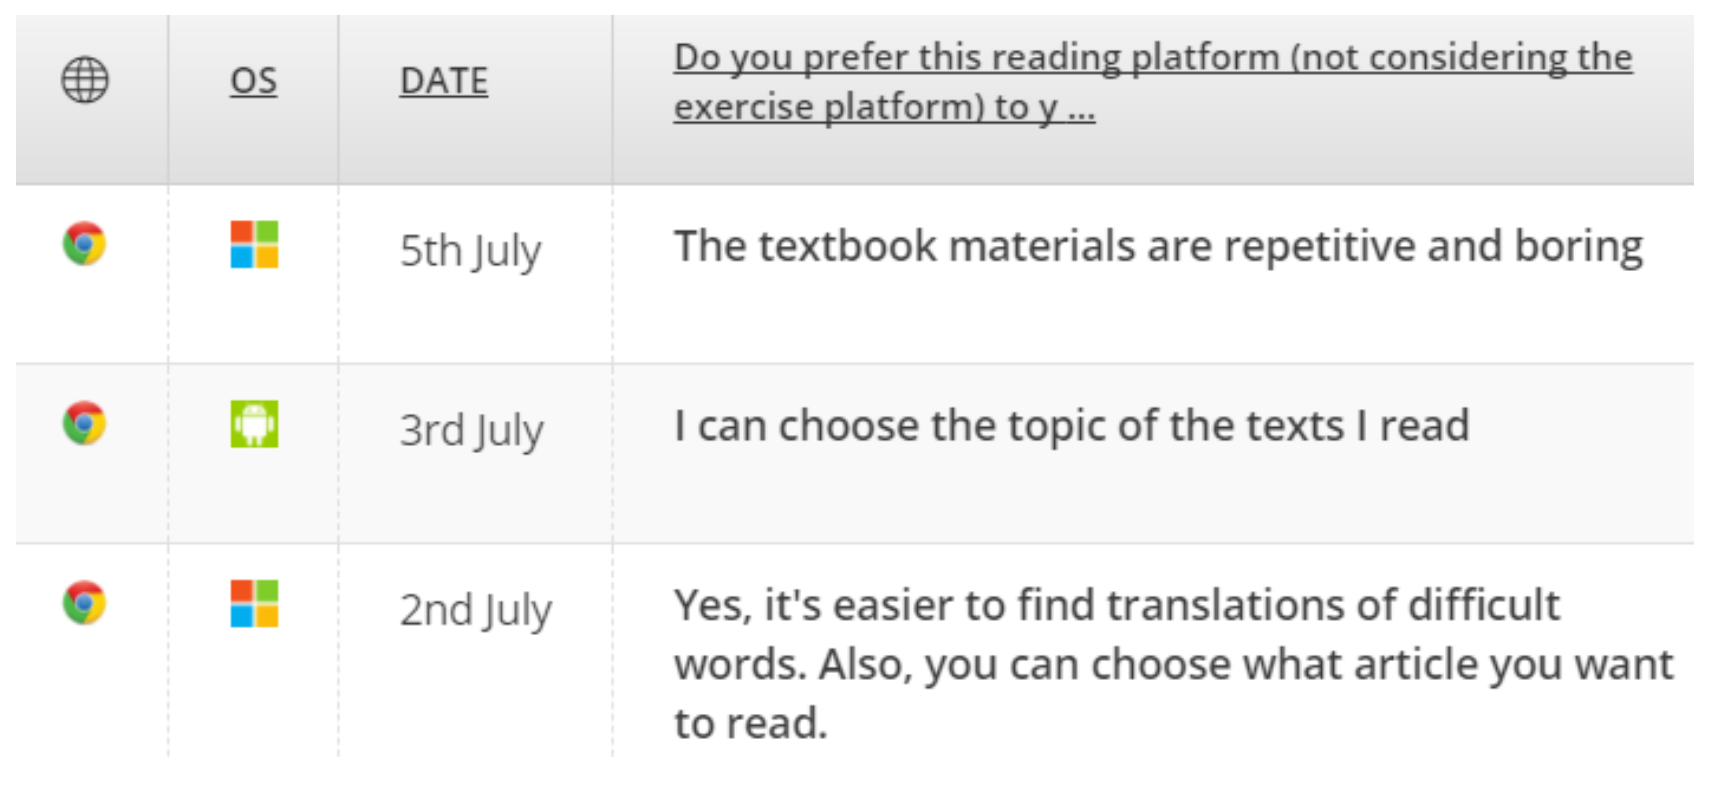
\includegraphics[width=0.9\columnwidth]{figures/opinion_on_reading_platform}
  \caption{The students appreciate the freedom of reading what is interesting to them }
\end{figure}

% \section{Acknowledgements}
% The authors would like to thank other contribu












% Balancing columns in a ref list is a bit of a pain because you
% either use a hack like flushend or balance, or manually insert
% a column break.  http://www.tex.ac.uk/cgi-bin/texfaq2html?label=balance
% multicols doesn't work because we're already in two-column mode,
% and flushend isn't awesome, so I choose balance.  See this
% for more info: http://cs.brown.edu/system/software/latex/doc/balance.pdf
%
% Note that in a perfect world balance wants to be in the first
% column of the last page.
%
% If balance doesn't work for you, you can remove that and
% hard-code a column break into the bbl file right before you
% submit:
%
% http://stackoverflow.com/questions/2149854/how-to-manually-equalize-columns-
% in-an-ieee-paper-if-using-bibtex
%
% Or, just remove \balance and give up on balancing the last page.
%
\balance{}

% BALANCE COLUMNS
\balance{}

% REFERENCES FORMAT
% References must be the same font size as other body text.
\bibliographystyle{SIGCHI-Reference-Format}
\bibliography{mir-biblio/aslan}

\end{document}

%%% Local Variables:
%%% mode: latex
%%% TeX-master: t
%%% End:
